\documentclass[9pt]{beamer}
\usepackage{beamerthemesplit} % new 
\usepackage{tcolorbox}
\usepackage{hyperref}
\usepackage{subfigure}
%\usetheme{Frankfurt}
\usetheme{Madrid}
%\usetheme{Copenhagen}

%Document begins
\begin{document}
\title{The Mathematical Mechanic} 
\author{Sushovan ``Sush'' Majhi}
%\date{\today} 
\date{September 8, 2015}
\frame{\titlepage} 

\begin{frame}
  \begin{center}
    
\includegraphics[scale=0.4]{feynman.jpg}
  \end{center}
\end{frame}

\frame{\frametitle{Overview}\tableofcontents} 

\section{Integrals Using Mechanics} 

\frame{\frametitle{Evaluating $\int_0^x\sin{t} dt$ Using Pendulum}
  Consider the two-dimensional simple pendulum,
  \begin{figure}
    \hfill
    \subfigure[Forces]{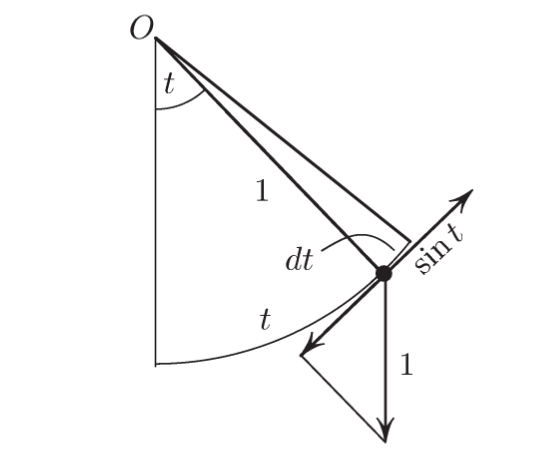
\includegraphics[width=5cm]{int_3.png}}
    \hfill
    \subfigure[Torque]{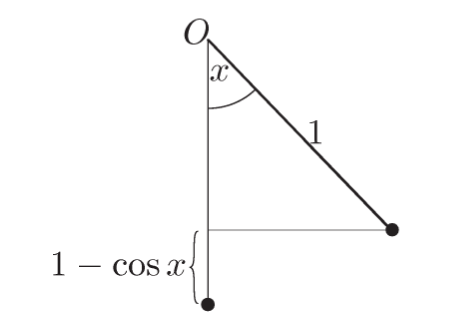
\includegraphics[width=5cm]{int_4.png}}
    \hfill
    \caption{2}
  \end{figure}
  
} 


\frame{\frametitle{Evaluating $\int_0^1\frac{x}{\sqrt{1-x^2}}dx$ Using Torque Balance} 
  Look at the mechanical structure below
\begin{figure}
  \hfill
  \subfigure[Forces]{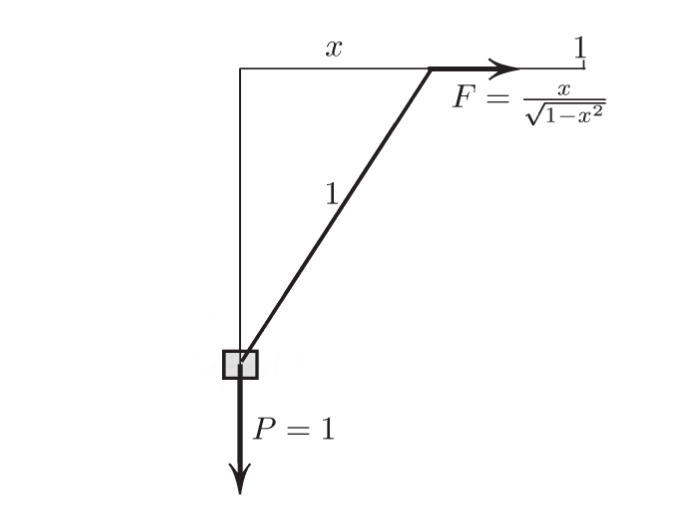
\includegraphics[width=5cm]{int_1.png}}
  \hfill
  \subfigure[Torque]{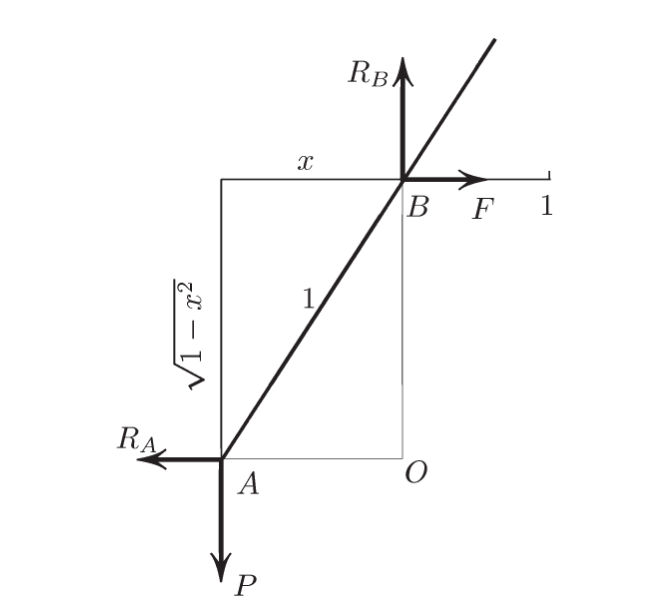
\includegraphics[width=5cm]{int_2.png}}
  \hfill
  \caption{1}
\end{figure}
}

\section{Complex Analysis And Fluid}

\begin{frame}
  \frametitle{Complex Functions And Vector Fields}
  \begin{block}{}
    $H:\mathbb{C}\to\mathbb{C}$ can be visualized as a steady two dimensional vector field 
    $X:\mathbb{R}^2\to\mathbb{R}^2.$
  \end{block}
  \pause
  \begin{block}{Polya Vector Field}
    For any complex valued function $H$ of a single complex variable, the vector field associated with $\bar{H}$ is called the 
    Polya vector field of $H$.
  \end{block}
\end{frame}

\begin{frame}{Polya Flows Of Complex Functions}
  \begin{center}
    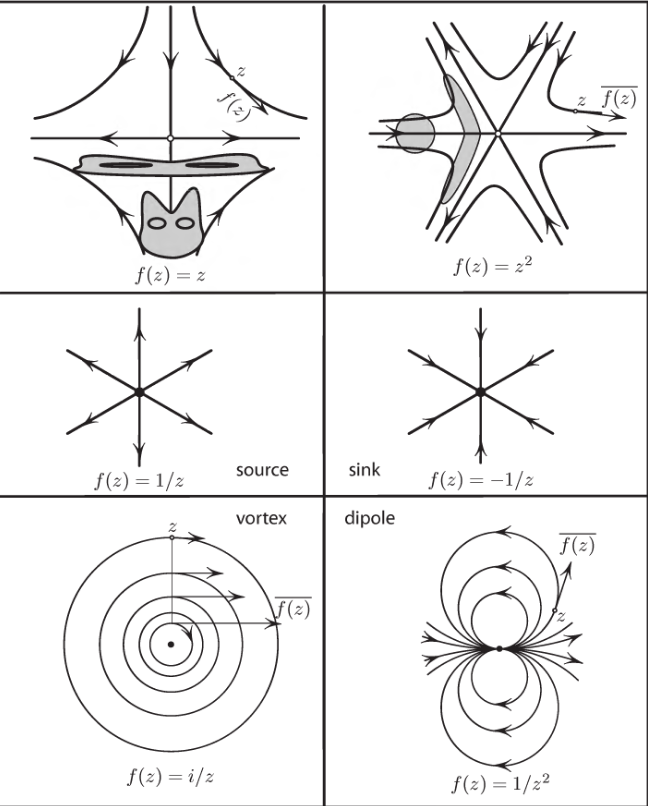
\includegraphics[scale=0.25]{flows.png}
  \end{center}
\end{frame}

\begin{frame}{Two Derivatives}
  \begin{block}{Divergence}
    $$\nabla\cdot X:=\frac{\partial X_1}{\partial x}+\frac{\partial X_2}{\partial y}$$\\
    Note: This quantity is invariant under coordinate transformation
  \end{block}
  \pause
  \begin{block}{Curl}
    $$\nabla\times X:=\frac{\partial X_2}{\partial x}-\frac{\partial X_1}{\partial y}$$\\
    Note: This quantity is invariant under coordinate transformation
  \end{block}
\end{frame}

\begin{frame}{Two Integrals}
  \begin{block}{Work Done, Ciculation}
    For any smooth curve $K$, 
    $$\mathcal{W}[X,K]:=\int_KX\cdot Tds$$
    This is a path/line integral.\\
    When $K$ is a closed curve, this has a special name, Circulation of $\bar{X}$ along $K$.
  \end{block}
  \pause
  \begin{block}{Flux}
    $$\mathcal{F}[X,K]:=\int_KX\cdot Nds$$
    It is a surface integral, in general. In our two-dimensional case it it a line integral.
  \end{block}
\end{frame}

\begin{frame}
  \begin{center}
    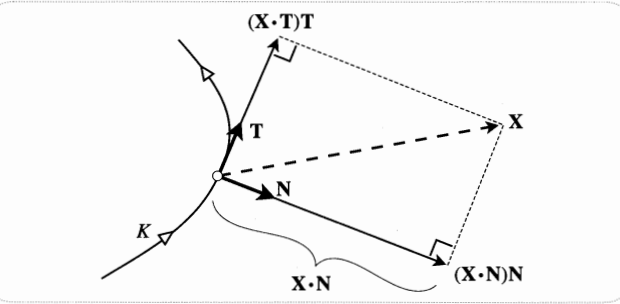
\includegraphics[scale=0.5]{integrals.png}
  \end{center}
\end{frame}  

\begin{frame}{How These Derivatives And Integrals Are Connected?}
  \begin{block}{Gauss Divergence Theorem}
    $$\mathcal{F}[X,K]=\int\int_R[\nabla\cdot X]dA$$
    where $R$ is the region encapsulated by the closed curve $K$. 
  \end{block}
  \pause  
  \begin{block}{Stoke's Theorem(Green's Theorem In Our Case)}
    $$\mathcal{W}[X,K]=\int\int_R[\nabla\times X]dA$$
  \end{block}
  
\end{frame}

\begin{frame}{Ideal Fluid Flow And Analytic Functions}
  \begin{block}{Ideal Fluid}
    A fluid flow is called an Ideal Flow if it is Curl-Free/Irrotational($\nabla\times X=0$) and 
    Divergence-Free($\nabla\cdot X=0$) at every point in the region where it is defined.\\
    As a consequence, for an ideal flow $X$, circulation and flux vanish around any closed curve in the domain.\\ 
  \end{block}
  \pause
  \begin{block}{CR-equations Vs Ideal Flow}
    CR-equations confirm that The Polya vector field of an analytic function is Ideal!\\   
  \end{block}
\end{frame}

\begin{frame}{Complex Integral In Terms Of Flux And Circulation}
  \begin{block}{Complex Line Integral Vs Polya Flow}
    Let $H:\mathbb{C}\to\mathbb{C}$ be a continuous complex function. Then,
    $$\oint_KH(z)=\mathcal{W}[\bar{H},K]+i\mathcal{F}[\bar{H},K]$$
    where $\bar{H}$ is the Polya vector field of $H$.
  \end{block}
 \end{frame}

\begin{frame}{Cauchy's Theorem Vs Ideal Fluid}
  Trivially true. 
\end{frame}

\begin{frame}{Evaluating Two Complex Integrals Using Physical Intuition}
  \begin{block}{An example}
    Let's calculate 
    $$\oint_K\bar{z}dz=2iArea(R)$$
    where $R$ is the region bounded by $K$.
  \end{block}
  \begin{center}
   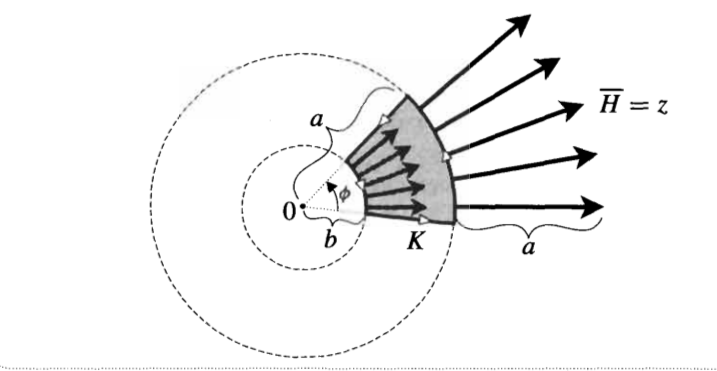
\includegraphics[scale=0.3]{example.png}
  \end{center}
\end{frame}

\begin{frame}{Cauchy Integral Formula Is Obvious!}
  \begin{block}{Theorem}
    Let $H:\mathbb{C}\to:\mathbb{C}$ be an analytic function then $$H(w)=\oint_K\frac{H(z)}{z-w}dz$$ where $K$ is a simple closed curve 
    enclosing $w$ in it's interior.
  \end{block}
  \begin{center}
    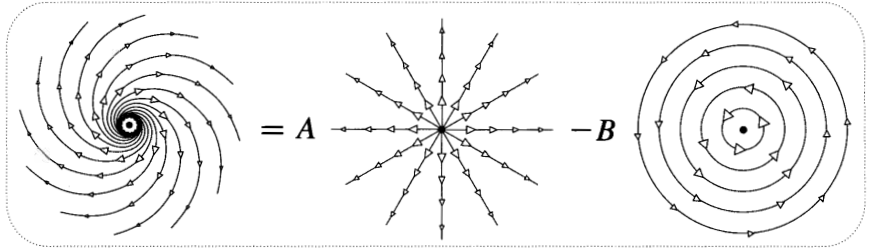
\includegraphics[scale=0.35]{formula.png}
  \end{center}
\end{frame}

\begin{frame}{Euler's Sum Via Fluid Flow}
  \begin{block}{Euler's Sum}
    $$\sum_1^\infty\frac{1}{n^2}=\frac{\pi^2}{6}$$ 
  \end{block}
  \pause
  \begin{block}{}
    Consider the Polya vector field of $$H(z)=\frac{\cot\pi z}{2z^2}$$
    \begin{center}
      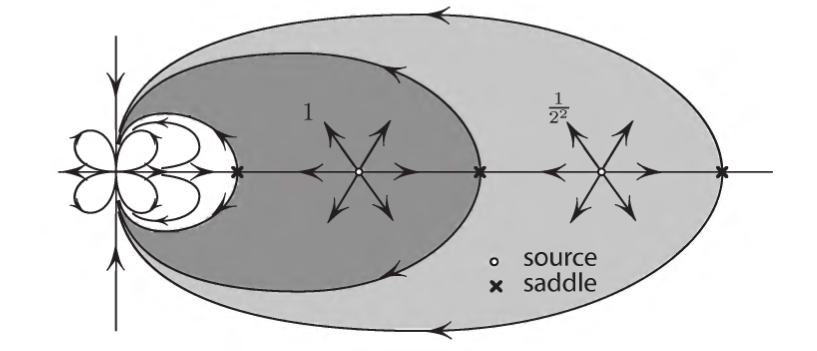
\includegraphics[scale=0.2]{euler.png}
    \end{center}
  \end{block}
\end{frame}


%% \section{Inequalities And Electricity}
%% \begin{frame}
%% \frametitle{AM$\geq$ GM}
%% abcd
%% \end{frame}

\begin{frame}{References}
  \begin{enumerate}[a.]
  \item ``The Mathematical Mechanic'', Mark Levi
  \item ``Visual Complex Analysis'', Needham
  \item ``Lectures On Physics, R. Feynman'', Vol 1,2 
  \end{enumerate}
\end{frame}
\begin{frame}
  \begin{center}
    \Huge Thank You!
  \end{center}
  
\end{frame}


\end{document}
